\begin{figure}[h]
	\centering
	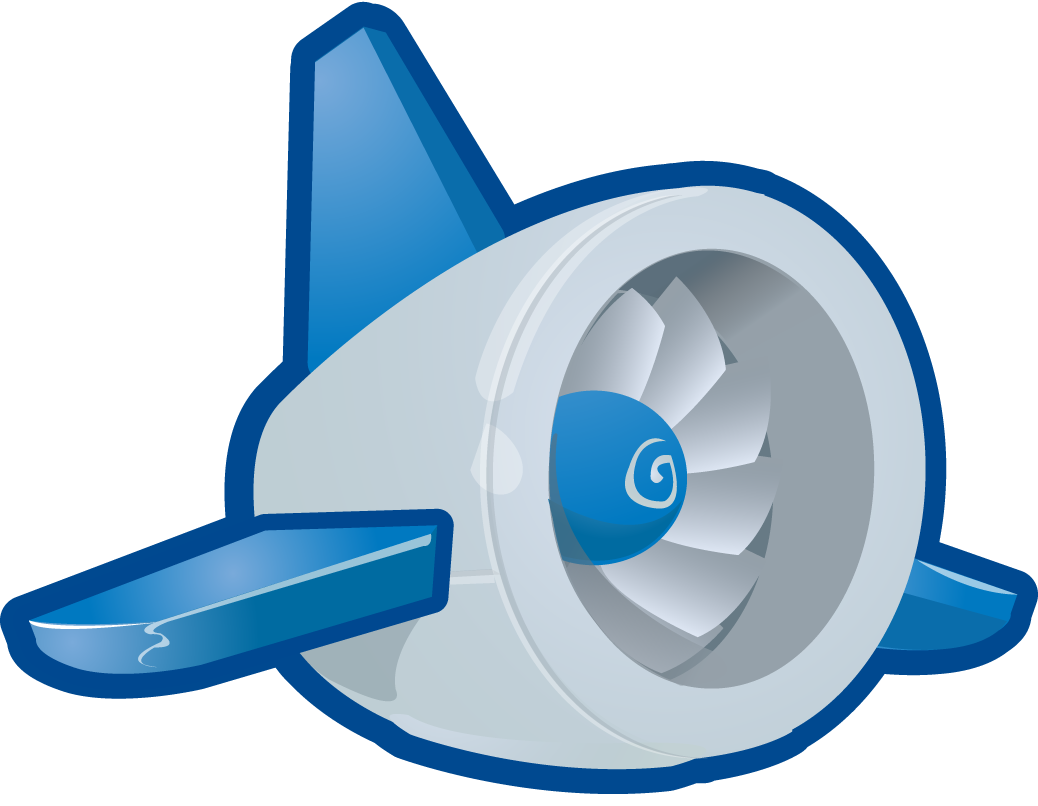
\includegraphics[scale=.25]{applogo}
	\caption{Google App Engine Logo}
	\label{Fig:applogo}	
\end{figure}

Google App Engine is a Platform as a Service (\textit{PaaS}) which allows users to build and run web applications on Google  infrastructure.

Thus, when a programmer writes a web application that runs on App Engine, the software is going to run on the Google servers, somewhere in the Google cloude \cite{UGAE}. This solution is very useful because allows everyone to write the own web program without purchasing and maintaining the needed hardware and network.

For the time being Google App Engine supports web applications written in a variety of the main programming languages for the web: \textit{Java}, \textit{Python}, \textit{PHP}, and \textit{GO}. Since the App Engine was first built in $2008$ for Python, this is the language used to carry out the web application for this thesis.

Over the possibility to create our own web application without dealing with hardware, the Google App Engine has been chosen because of its datastore and memcache, which allow a simple memorization of data, automatic scaling and load balancing, and more others important features that are going to be shown below.

To create a more scalable and hierarchical web application the \textit{Flask framework} has been used. Flask is a lightweight web application framework written in Python. It is based on the \textit{WSGI} toolkit and Jinja2 template engine and it is distributed with a \textit{BSD} license.\\ Flask provides an easy way to organize a web application which allows to build up complex website easy to manage. It has no database abstraction layer, indeed for this purpose, in this application, it supports the Google App Engine.

\begin{figure}[h]
	\centering
	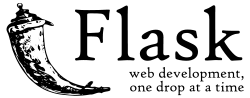
\includegraphics[scale=.8]{flask}
	\caption{Flask Logo}
	\label{Fig:flasklogo}	
\end{figure}